%!TEX root = ../../ClassicThesis.tex


In this chapter, we present background information which the reader is required to know in order to understand the original research material which follows in the remainder of the thesis.
Here, we will introduce and discuss the fundamental properties of the mammalian visual system, information theory, and neuronal correlations.


%------------------------------------------------------------------------------
\section{Neurons and the brain}

The central nervous system consists of the brain, spinal cord, and retina.
Within each, there are specialised biological cells called \termemph{neurons}, whose properties allow them to encode information about the external world gleamed through the body's sensory organs, manipulate this information and perform computations with it in order to control the behaviour of the body.%
\footnote{
Neurons are common across all species of animals, though the architecture of their nervous systems vary greatly.
Plants are also able to infer properties of their environment and respond accordingly using chemical and electrical signals, despite their lack of neurons \citep{Brenner2006,Barlow2008}.
}
The peripheral nervous system and the retina together provide a stream of data about the environment within which the subject resides, known as the \termemph{senses} (sight, sound, touch, smell, taste, temperature, pressure, \textit{etc.}).
The computations performed by the central nervous system allow it to extract features from this stream of sensory information, store properties of it for later computational use, and decide which behavioural actions to perform in order to move its body and influence the environment within which it resides (arguably the only important function of a brain; \citealp{WolpertTED}).

Information transmission between neurons is principally mediated by changes in the voltage, or potential difference, between the inside and the outside of the neuron \citep[Chapter~2]{nsbook}.
A change in this membrane potential within one neuron will propagate along its cell body, and in doing so will affect other neurons which make direct conductive connections with it.
However, the majority of connections between neurons are indirect, involving a synaptic junction in which chemicals, referred to as neurotransmitters, are released by one neuron and sensed by another where it induces an electrochemical change.

In order to be able to transmit electrical signals over long distances (longer than \SI{1}{\milli\metre}), neurons digitise their information as \termemph{action potentials}.
At rest, the membrane potential of a neuron is typically negative, around \SI{-70}{\milli\volt}.
For an action potential to be elicited by a neuron, its membrane potential must depolarise, becoming less negative.
Once the membrane voltage passes above a certain threshold (typically around \SI{-55}{\milli\volt}, but the specific value depends on the neuron in question) a temporary change occurs in the dynamics of the ion channels which allow ionised chemicals to pass between the inside and outside of the cell.
Sodium ions suddenly flow into the neuron, then potassium ions flow out just as suddenly, causing the membrane potential to rapidly increase to around \SI{+40}{\milli\volt} and then fall back to a voltage a little below its value at rest.
The sharp rise and fall of the voltage across the membrane is known as an action potential, or \textemph{spike}, and has a duration of only around \SIrange{1}{2}{\milli\second} \citep[Chapter~1]{Dayan2001}.
Following a spike, there is a recovery period (refractory period) of another few milliseconds during which further spikes cannot be elicited; following this the system is returned to its original resting state.

We can consider an occurrence of action potential event to be the output of a neuron.
Aided by an insulating covering of myelin and repeating stations (known as Nodes of Ranvier), an action potential can travel along its \termemph{axon} for long distances.%
\footnote{
% The longest neuron in the human body is the sciatic nerve, which stretches from the base of the spine to the big toe.
The longest axon in the human body is the that of the dorsal root ganglion, which extends from the big toe to the primary sensory cortex in the brain.
The equivalent nerve in the blue whale can have an uninterrupted axon \SI{25}{\metre} in length \citep{Smith2009,Voytek2012}.
}
At the terminus of the axon, synaptic connections are formed with the dendrites of other neurons.
Upon the arrival of an action potential at the synapse, neurotransmitters are released which can either increase or decrease the membrane potential of the recipient neuron.

Learning occurs principally by the strengthening and weakening of these synaptic connections between neurons such that more or fewer neurotransmitters are transferred into the recipient upon the arrival of a single action potential (\citealp[Chapter~8]{Dayan2001}; \citealp[Chapter~23]{nsbook}).


%------------------------------------------------------------------------------
\section{Mammalian visual system}
\label{sec:bg_visual_system}

Sensitivity to the visual spectrum is an important survival trait for almost all land animals.
Whether predator or prey, the ability to see allows an individual organism to receive and perceive information about their environment over large distances.
Such a trait has obvious survival implications, and therefore confers an evolutionary advantage.

\begin{figure}[htbp]
\centering
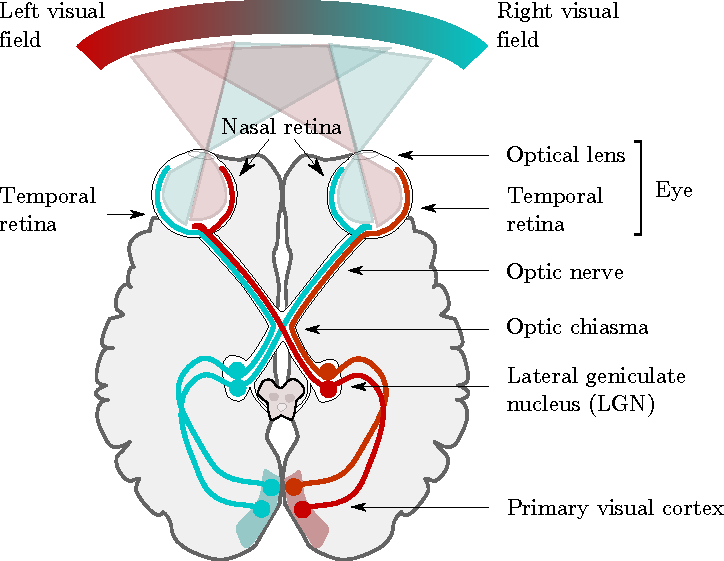
\includegraphics[scale=.9]{Human_visual_pathway.pdf}
\caption{%
\captionemph{Human visual pathway.}
Visual information enters the eye, is encoded in the retina and progresses to the visual cortex, via the \ac{LGN}.
Reproduced (with modifications) from \href{https://commons.wikimedia.org/wiki/File:Human_visual_pathway.svg}{Wikimedia Commons} under the \href{https://creativecommons.org/licenses/by-sa/4.0/deed.en}{CC BY-SA 4.0} license.
}
\label{fig:bg_visual_pathway}
\end{figure}

Across all mammals, the visual system is composed of several processing stages, illustrated in \autoref{fig:bg_visual_pathway}.
Light enters the eye (if possible, focused into a clear image by the lens), and is encoded as electrical signals in the retina at the back of the eye.
This information is transmitted to the brain through the optic nerve, where it reaches the \ac{LGN}.
From here, the visual information is propagated to the \acf{V1}, which feeds its outputs to the rest of the visual (and non-visual) cortical regions.
For humans and other primates, vision is our dominant sense, and a large fraction of our brains (sometimes estimated as around half the brain, excluding the cerebellum) is devoted to processing visual information.


\subsection{The eye}

The story of visual perception begins with the eye.
Eyes have evolved multiple times throughout the history of life on Earth.
Noting that other animals have eyes which are structured differently, in this section we describe the properties of the eye as they are for humans and other mammals.


\subsubsection{Rods and cones}

For any visual system, the most fundamental component is a set of cells which are sensitive to electromagnetic radiation.
In mammals the light-sensitive cells, or \textemph{photoreceptors}, come in two types: \termemph{rods} and \termemph{cones} \citep[Chapter~11]{nsbook}.%
\footnote{
There are also intrinsically photosensitive \aclp{RGC}, however these cells are not directly involved in forming an image of the visual stimulus.
Instead, they mediate the circadian rhythm, and influence pupil dilation \citep{Berson2002,Ecker2010,Wong2005}.
}
Rods and cones are subtypes of neurons which contain photosensitive proteins, rhodopsin and photopsin, respectively.
When photons of light collide with a photopigment protein, it changes state and shape, causing a cascade of biochemical changes resulting in the closing of ion channels in the cell membrane of the neuron.
Since the energy in the photon%
\footnote{
The amount of energy within a photon is related to its wavelength according to the Planck--Einstein relation,
$E = h f$, where $E$ denotes the energy of a photon, $f$, the frequency associated with it, and $h$ is Planck's constant.% h = 6.626...\times 10^{−34}
}
(which is indivisibly quantised) must closely match the difference in energy levels of the photopigment, each photopigment is only sensitive to a particular range of wavelengths of light.
The spectral absorption curves for photopigments used in the rods and cones of humans are shown in \autoref{fig:bg_cone_responses}.

\begin{figure}[htbp]
\centering
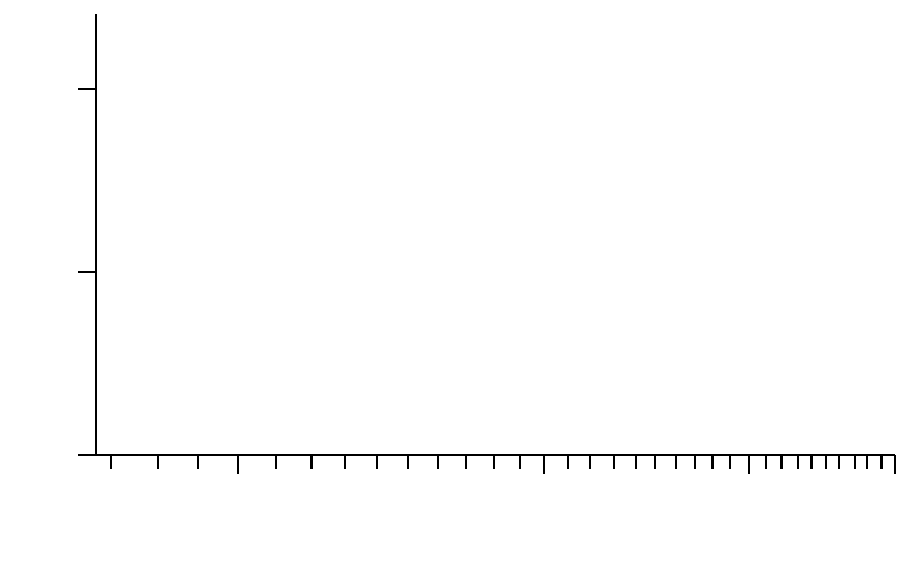
\includegraphics[scale=.625]{Cone-response.pdf}
\caption{
\captionemph{Spectral absorption curves for pigments found in cone and rod cells.}
The normalised response curves for \aclp{R} (\acsu{R}) and \acf{L}, \acf{M}, and \acf{S} cones typical of humans with normal colour vision.
Note the $x$-axis scales linearly with frequency, and hence is non-linear with respect to wavelength.
Beneath, the common names of the visible colours are indicated at their respective frequencies.
Reproduced (with modifications) from \href{https://commons.wikimedia.org/wiki/File:Cone-response.svg}{Wikimedia Commons} under the \href{https://creativecommons.org/licenses/by-sa/3.0/deed.en}{CC BY-SA 3.0} license, showing data appearing in \citet{Bowmaker1980}.
}
\label{fig:bg_cone_responses}
\end{figure}

Rod photoreceptor cells are very sensitive to light, making them ideal for seeing in dark and low-lighting conditions.
% These cells have a large surface area over which the photopigment is exposed to light, and their photopigment is very sensitive, producing a high gain on the detected signal.
However, in well-lit scenes, rods quickly become saturated, at which point they offer no information about the external world other than the fact that it is ``quite bright right now''.

Cone photoreceptors come in several different types, each using a different photopigment to detect different ranges of the electromagnetic spectrum.
In humans, there are three types%
\footnote{With the exception of colour-blind individuals, who may have only two or fewer types of cones, and tetrachromats \citep{Nagy1981,Jordan1993,Jameson2001} who have four.}
of cones:
\acl{L}, \acl{M}, and \acl{S} (\acsu{L}, \acsu{M}, and \acsu{S}) cones.
These can be approximately considered sensitive to red, green, and blue light respectively --- however, it should be noted that there is a broad range of wavelengths which each is sensitive to (see \autoref{fig:bg_cone_responses}), and this range is very similar for the \ac{L} and \ac{M} cells.
Possessing three cones makes humans (along with other apes and Old World monkeys) the exception instead of the norm within the mammal class --- most mammals, including cats, dogs, and the New World monkeys, are dichromatic with only two types of cones (\ac{M} and \ac{S}).

The presence of photoreceptors with different spectral sensitivities enables \textemph{colour vision}.
When light of a given frequency meets the retina, we can compare the relative responses of the different types of cone to determine which frequency it was.
From the absolute intensity of the responses, we can determine the intensity or brightness of the light.

The distribution of rods and cones within the eye is not uniform.
Across most of the eye, the density of rods is twenty times higher than that of cones; however, there is a small region of \SI{1.2}{\milli\metre} diameter, called the \termemph{fovea}, within which the cone density is \num{200} times higher \citep[Chapter~11]{nsbook}.
The extremely high cone density within the fovea, which covers the central \SI{5}{\degree} of the visual field, provides this part of the retina with the highest visual acuity.
To preserve the high resolution of foveal vision, in this small part of the retina there is a one-to-one mapping from cones to bipolar cells, and \numrange{3}{4} times more ganglion cells than cones \citep{Wassle1990}.
% Light reaching the fovea originates directly from the direction of fixation of the eyes.

The very highest level of visual acuity is in the foveola --- the central part of the fovea where the cone density is greatest --- which covers eccentricities less than \SI{0.5}{\degree} from the line-of-sight \citep{Hendrickson2005}.
Surrounding the fovea, is the parafovea which includes eccentricities from \SIrange{2.5}{4}{\degree}.
This, in turn, is encomposed by the perifovea, extending out to \SI{9}{\degree} of eccentricity.
The rest of the visual field is referred to as peripheral, and has coarser acuity.
Visual acuity decreases greatly away from the fovea; with an eccentricity of just \SI{6}{\degree} from the line of sight, acuity falls to \SI{25}{\percent} of its peak \citep[Chapter~11]{nsbook}.
Consequently, humans move their eyes (and heads) frequently to ensure they can see the subject of their attention as clearly as possible even as their attention shifts between subjects.

Throughout the rest of the eye, the high density of rods ensures that the few photons which are present in low-lighting conditions have as a high chance of meeting a rod cell as possible.
Even so, only \SI{10}{\percent} of the photons which reach the eye are absorbed by a rod \citep{Hecht1942}.

The ratio of the three types of cones is also neither balanced nor homogeneous across the surface of the retina.
Although the proportion of \ac{M} and \ac{L} cones are roughly equal, \ac{S} cones constitute only \SIrange{5}{10}{\percent} of the total, and even less within the fovea \citep[Chapter~11]{nsbook}.
This provides humans with excellent ability to distinguish between shades of red, orange, yellow, and green, and is thought to have been evolutionarily selected for in order to enhance the ability to spot fruit in bushes \citep{Bompas2013}.


\subsubsection{Retinal processing}
\label{sec:bg_retinal_processing}

Since there are about \num{130} million photoreceptors in the human eye, but only \num{1.5} million axons which send information from the retina to the brain \citep{Nassi2009}, the information collected from the photoreceptors must be compressed.
This compression is lossy, but the processing performed in the retina allows the important properties of natural stimuli to be preserved and unimportant properties discarded.
The important feature of natural stimuli which must be preserved is the spatial variations in luminance \citep[Chapter~11]{nsbook}.
Indeed this is the reason why there are so many photoreceptors in the first place --- to capture spatial changes at high resolution.
One unimportant feature of the stimuli is the absolute intensity of the light; consequently the output from the retina to the brain is local spatial contrast and how this varies over time.
Furthermore, the colour of stimuli tends to vary coarsely within stimuli, and so this is downsampled.
There is also decorrelation of the output from the retina, reducing the redundancy in the information sent to the brain.

This functionality is achieved by the circuitry within the retina.
In particular, \termemph{bipolar cells} connect to the rods and cones and filter their outputs, with some bipolar cells inverting the output of the photoreceptors.
\acused{RGC}
\termemph{Retinal ganglion cells} (\acsp{RGC}) connect to a group of these bipolar cells, connected such that each \ac{RGC} has a small, localised, circular \ac{RF} to which it is sensitive.
Each \ac{RGC} is wired such that they are sensitive to the difference in intensity between the centre of their \ac{RF} and the rest of the \ac{RF}.
Consequently there are two complementary flavours of \acp{RGC}.
The first responds strongly when the centre of the \ac{RF} is more illuminated than the surrounding (an \termemph{on-centre} ganglion), and the second responds strongly when the surrounding is more illuminated than the centre (an \termemph{off-centre} ganglion).
The axons of the \acp{RGC} constitute the optic nerve, and their outputs are the source of visual information received by the brain.

Invariance to the changes in absolute illumination is produced partly by the centre-surround selectivity of the \acp{RGC}, and partly by \termemph{horizontal cells}.
Horizontal cells receive inputs both from several cones and from other horizontal cells, such that each has a wide \ac{RF} and represents the average illumination over a large area \citep[Chapter~11]{nsbook}.
The output of horizontal cells is fed back to the cones, suppressing their changes in activity driven by illumination.
In doing so, horizontal cells effectively subtract from each cone the average activity of all neighbouring cones, providing light adaptation.

There are known to be many types of \acp{RGC} (at least \num{17}), most of which are not well studied and poorly understood, but the three most common types are well characterised and constitute around \SI{88}{\percent} of all the \acp{RGC} \citep{Nassi2009}.

Midget ganglion cells have small receptive fields with low contrast sensitivity and consequently sensitivity to high spatial and low temporal frequencies \citep{Nassi2009}.
They are red-green colour opponent, with either an \ac{M} or \ac{L} cone in the centre and a mixture of \ac{M} and \ac{L} cones surrounding it.
Approximately \SI{70}{\percent} of retinal cells which project to the \ac{LGN} are midget cells, making them by far the most common class of \acp{RGC}.

Parasol ganglion cells have larger receptive fields, resulting in higher contrast sensitivity which is achromatic, and a preference for high temporal, low spatial frequencies \citep{Nassi2009}.
The axon conductivities for parasol ganglion cells are higher than those of midget ganglions, and output of the parasols provides the first visual response within the visual cortex.

The third most common \ac{RGC} type is the bistratified ganglion cells, which convey blue-on yellow-off colour-opponent signals.

% Each type of \ac{RGC} is tiled across the retina.


\subsection{The \acl{LGN}}

The optic nerve sends visual information from the retina to the \acf{LGN}.
The \ac{LGN} is banded, with layers of cells of several types, as illustrated in \autoref{fig:bg_pathway}.

\begin{figure}[htbp]
\centering
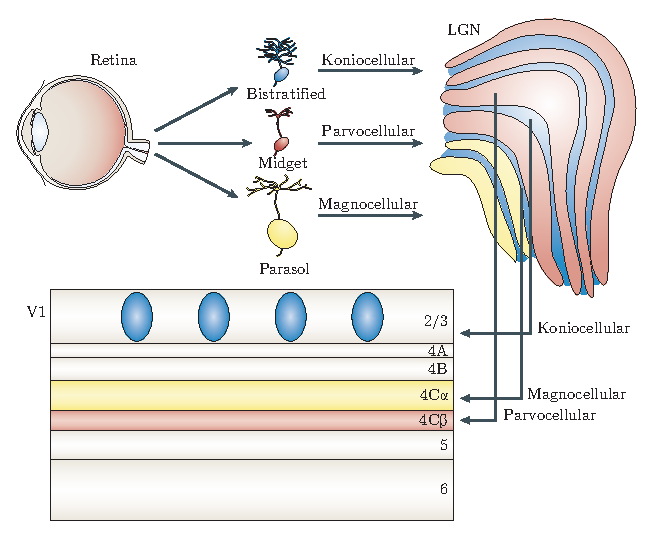
\includegraphics[scale=1.25]{Nassi2009_fig2.eps}
\caption{
\captionemph{Parallel pathways from the retina to the cortex.}
Midget (red), parasol (yellow), and bistratified (blue) ganglion cells are well characterized and have been linked to parallel pathways that remain anatomically separate through the \ac{LGN} and into the \ac{V1}.
Although these ganglion cell types are numerically dominant in the retina, many more types are known to exist and are likely to provide other important pathways yet to be identified.
Adapted by permission from Macmillan Publishers Ltd: \textit{Nature Reviews Neuroscience} \citep{Nassi2009}, copyright 2009.
}
\label{fig:bg_pathway}
\end{figure}

The outputs of midget \acp{RGC} are directed to parvocellular layers in the \ac{LGN}, which is then directed to \aclu{L4Cb} within \ac{V1} (\acs{L4Cb}).
Because the signal passes through the parvocellular layers, this is known as the P-pathway.
Parasol \acp{RGC} target the magnocellular \ac{LGN} layers, which subsequently target \acs{L4Ca} of \ac{V1} (the M-pathway).
Bistratified \acp{RGC} project to the koniocellular layers of \ac{LGN}, which then target cytochrome oxidase-expressing patches (blob cells) in \aclu{L2/3} of \ac{V1} (\acs{L2/3}; the K-pathway).

The tuning properties of \ac{LGN} cells are very similar to \acp{RGC}.
Each of these three streams progresses simultaneously and in parallel, conveying different information about the stimulus but sampling from the same spatial locations within the visual field.


\subsection{The primary visual cortex}
\label{sec:bg_v1}

The \acf{V1} is constituted of several \termemph{layers} stacked on top of each other, with total thickness around \SI{2}{\milli\metre} in primates.
Each of these layers contains a different distribution of the many types of cortical neurons, and each layer has inputs and outputs directed to different brain regions \citep{Harris2013}.
Classically, we refer to \num{6} anatomically-defined layers which together make up \ac{V1} --- however as knowledge about the cortical structure has increased, these have been subdivided further.

Fixing our location within the cortical plane and examining the properties of neurons as we move along the cortical depth reveals that these neurons have the same visual \ac{RF} (\citealp{Hubel1962}; \citealp{Hubel1963}), and this extends for a planar radius of around \SI{500}{\micro\metre} \citep{Mountcastle1997}.
Furthermore, the neurons within a cylindrical column of the cortex preferentially to oriented edges with the same angle \citep{Hubel1962}.
The structure of the cortex (the constitution of each of the \num{6} layers) is similar across all its planar surface (not just within the confines of area \ac{V1}), suggesting there is a fundamental columnar processing unit which is replicated across the surface of the cortex \citep{Mountcastle1957,Douglas1989,Douglas1991,Douglas2004,Binzegger2009}.
It has been hypothesised that the circuitry of the cortical column has structural and functional similarities across all sensory modalities, serving as a generic cortical processing unit.

Cortical columns (and their constituent neurons) within \ac{V1} have been observed to be tuned to bars or edges with specific spatial frequency, orientation, direction of motion, and colour.
Neighbouring cortical columns compete with each other due to the horizontal inhibition within \acs{L2/3} of \ac{V1}.
As a consequence, topological maps self-organise across the surface of \ac{V1}, together providing an efficient representation of the space of stimuli native to the individual's sensory environment \citep{Miikkulainen2005,Stevens2013,Wilson2015}.
As we traverse the cortical plane, neurons change in \ac{RF} location, preferred orientation, and spatial frequency, such that there is good coverage over the full distribution of possible stimuli.

However, it should be noted that the rate of change of \ac{RF} location is not constant as we traverse across the surface of \ac{V1}.
The very high density of cones within the fovea, and the one-to-one correspondence of cones to \acp{RGC} exclusively within the fovea, result in a disproportionately high fraction of the visual information reaching \ac{V1} originating at the fovea.%
\footnote{Approximately half the fibres in the optic nerve carry information from the fovea, despite the fact it only covers \SI{0.1}{\percent} of the eye's total field of view.}
Correspondingly, a larger fraction of cortical computation is expended on this region of the visual field, and the amount of cortical material devoted to processing foveal stimuli is higher than that devoted to peripheral stimuli.
The relationship between the eccentricity of an area within the visual field and the area within the visual cortex which is sensitive to this space is referred to as \termemph{cortical magnification}.
The amount of cortical magnification of the visual field is inversely proportional to the eccentricity from the foveola \citep{Strasburger2011}.


\subsection{The rest of the visual cortex}

From \ac{V1}, the flow of visual information within the brain forks, progressing down two parallel streams \citep{Goodale199220,Mishkin198257}.
Beginning with \ac{V1} and \ac{V2}, the dorsal stream progresses to \ac{V5} and \ac{V6}.
Brain regions within this stream are involved in spatial attention.
They communicate with other regions which control eye movements and hand movements, and hence it is nicknamed the ``where'' pathway.

The ventral stream also begins with \ac{V1} and \ac{V2}, but then progresses to \ac{V4} and the \acf{IT}.
Involved in the recognition, identification, and categorization of visual stimuli, it is referred to as the ``what'' pathway.
Whilst \ac{V1} responds strongly to oriented bars, neurons in \ac{V2} and \ac{V4} have been found to respond to increasingly more abstract shapes.
At the higher end of the visual stream, \ac{IT} contains cells which have been identified to respond to high-level objects, such as faces.%, and concept cells \cite{Quiroga2012}.

These visual cortical regions are connected to other cortical regions higher up the cortical processing hierarchy.
Some of these are associative cortical regions, which integrate information across different sensory modalities.
The visual and associative cortices are also connected to regions related to planning and decision making, such as the \acf{PFC}.


%------------------------------------------------------------------------------
\section{Information theory, and its applications within neuroscience}
\label{sec:bgit}

A common experimental methodology used in neuroscience is to record the extracellular activity of individual neurons under different conditions.
From this, we can compare the activity of the neuron under different conditions to examine whether it is dependent on this set of conditions, and if so investigate the nature of the relationship between the two.

Frequently, the approach used is to take many recordings of the same neuron for the same condition, and then take the average across these repetitions (\textemph{trials}) to reduce the effects of neuronal variability, producing a \ac{PSTH}, for instance.
This neuronal variability is often referred to as \textemph{noise}, however it is debatable as to whether differences in the behaviour of individual neurons between trials are due to noise within the system or are in fact due to non-stationarity within the system due to changes in neural state or unknown latent variables within the system (see \autoref{sec:bg-noisecorr} for further discussion).

Such a simple treatment of the data --- averaging the response over repetitions --- is fundamentally flawed, since this is not the manner in which brains process stimuli.
At any moment in time, the brain has access to the activity of many neurons simultaneously (not a single neuron in isolation), but only has a single sample of each one (not multiple instantiations of the same neuron).

If we instead use information theory to study the neuronal activity, we can consider how much information there is across a system containing multiple neurons during an isolated period of time, for instance a single trial.
By using an information theoretic technique, we can overcome the limitations of the more simple methods; but no method is perfect and there are other limitations which arise when using information theory instead.
In this section, I will first outline the analytic procedure through which information theoretic analysis is applied to neuroscientific data, some of the problems which arise, and how to try to overcome them.


\subsection{Neuroscientific context}

In the context of trying to experimentally investigate properties of the sensory cortex of the brain, one typically uses an experimental set-up with a finite collection of discrete experimental stimuli.
These stimuli are then repeatedly presented to the sensory organ in an appropriate fashion, and the responses during each presentation are recorded.

For such an experimental set-up, let us assume that on each trial some stimulus $s$ is selected at random, with probability $p(s)$, from a set of discrete stimuli $\SET{S}$.
The random variable $S$ denotes this selection of a stimulus, with some arbitrary probability distribution across the elements of $\SET{S}$.
Even if our stimuli come from a continuous stimulus space, parametrically varying in orientation or frequency, say, it is important to discretise this down to a finite subset of stimuli from which samples will be drawn.
This is because we must estimate either $p(s,r)$, $p(r|s)$, or $p(s|r)$ from the data for each stimulus $s$ and response $r$ in order to compute the mutual information, which is only possible if we have at least one presentation of every stimulus within our collection of stimuli.

The neuronal response could be one (or more than one) of several data types, such as a spike train from one or more neurons, the \ac{LFP}, \ac{CSD}, \ac{BOLD} signal, a calcium indicator, \ac{EEG}, or others \citep{Magri2009,Quiroga2009}.
The principles of information theory can be applied whichever neural signal recorded from and taken to be a measure of the neural response.
In \autoref{ch:pl}, we will work with information encoded in \ac{MUA} and spike trains, whilst in Chapters~\ref{ch:lam} and \ref{ch:plam} we will be considering the \ac{LFP} and \ac{CSD}.

With regards to the analysis of sensory recordings (with which this thesis will be concerned), the different conditions used on the trial are typically different stimuli, and the extracellular recordings provide us with the neuron's response to the stimuli.
When applying information theory to neuronal data, we treat the brain as a communication channel, transmitting information about sensory input.
We are hence interested in how much information the response in the brain contains about which stimulus was presented to it.

However, it should be noted that we frame the problem in the context of a \termemph{communication channel} simply because this is the framework around which Shannon information is formulated \citep[Chapter~2]{mackay2003information}.
Within information theory, systems are modelled with information passing between a transmitter and receiver through a communication channel.
The message passing between them is modified as it passes through the channel, and the receiver must attempt to decipher which message was originally sent.

In some ways, some functions of the brain are similar to the process of a compression algorithm.
The initial encoding of the stimulus as transcribed by the appropriate sensory organ contains a large amount of information about the precise input stimulus --- for example the individual pixel values with an image stimulus --- which has a large amount of redundancy if one is interested only in detecting, classifying, and reacting to stimuli.
A binary image of only $17 \times 17$ pixels can express \num{9.9e86} different states --- a value ten million times larger than the number of atoms in the visible universe, thought to be around $10^{80}$.
However the vast majority of these images (for this, and equally true for a larger image with more intensity levels and colours) resemble unstructured random noise.
The set of images which are of interest for interacting with a real world environment is vastly smaller; with an appropriate high-level statistical model, the subset of stimuli which are of interest can be compressed down to a much smaller number of bytes.
For instance, we can take large image and compress this down to a binary value indicating whether this visual stimulus contains the face of familiar person.

After a stimulus has been processed by the brain, information about the exact intensities of individual pixels is lost, but salient information about the environment is preserved.
We can hence investigate how stimuli are encoded within the brain by considering certain properties of the stimulus and computing the amount of information about them which is contained within the neural recordings.
Here, we make the following assumption: if the neuronal activity is observed to contain information about the stimulus, we can assume this information is present due to the manner within which information is encoded by the brain, and that this information can be drawn upon to inform decisions taken with regard to the stimulus.
We rationalise this assumption on the basis that we know the brain contains information about stimuli (otherwise it would be functionally blind/deaf), and it would be wasteful to expend resources encoding stimuli accurately but in a non-functional manner.
Such waste would run contrary to the evolutionary pressures for energy efficiency within the neuronal architecture \citep{Laughlin2001,Niven2008}.

The neural data which can be collected with modern experimental equipment is very dense and rich in content.
For instance, individual spikes can be recorded with the precision of fraction of a millisecond, and broadband \acp{LFP} allow for many frequency components to be analysed from the same recording.
Typically, it is not possible to compute the information about the stimulus contained in the entire data stream all at once when such a large quantity of neural activity is recorded simultaneously.
This is because our analysis is limited by the relatively small number of trials which can be collected for any given dataset.

% Mark dislikes this paragraph I guess?
In order to study information encoded within neural recordings, we must compare the activity across many repetitions of the same stimulus.
Furthermore, to be able to compare the activity across trials, we must ensure we are making our recordings in precisely the same manner throughout all trials.
Given the large number of neurons within the brain and the natural movement of brain tissue over time, it is not possible to set-up multiple experiments with the same subject and record precisely the same neurons each time.
Consequently, the maximum number of repetitions we can achieve for any recording stream is limited to the number of repetitions which can be recorded over the course of a single recording session of at most a few hours in duration.
With trials whose duration are in the order of a minute, we can only expect to record in the order of 100 trials in any dataset with consistent and comparable neural recordings across all the trials.

Using information theory, we can investigate the nature of the neural code used by individual neurons and populations of neurons \citep{Optican1987}.
For example, if our dataset consists of recordings of neuronal spiking activity, we can consider the amount of information contained in the spike train coincident with a \SI{40}{\milli\second} stimulus, say.
First, we can consider our response vector to be the total number of spikes over the \SI{40}{\milli\second} window and compute the information contained in these about the identity of the presented stimulus.
Second, we can consider our response vector to be the number of spikes in each quarter of the stimulus presentation period (four \SI{10}{\milli\second} windows).
This step could equally be performed with more windows of finer granularity, so in general we would have a response vector $r = [r_1, \ldots, r_L]$, with $L$ windows each of length $\nicefrac{T}{L}$ and $r_i$ the number of spikes during the $i$-th window\footnote{In our example, $T = \SI{40}{\milli\second}$.}.
Since the information contained in single \SI{40}{\milli\second} window approach is, by construction, fully contained in the vector of responses within the shorter windows, we can investigate amount of information contained within the timing of the spikes.
If there is no significant difference between the amount of information about the stimulus contained in the two vectors, it seems reasonable to conclude that the stimulus, or some attributes which distinguish it, are encoded in the firing rate, whilst the exact timing of the spikes is unimportant.

% Typically \citep{Quiroga2009,Brasselet2012,Panzeri2007,Arabzadeh2006,Strong1998}, a certain post-stimulus time window of duration $t$ in \SIrange{20}{40}{\milli\second} is chosen and a neural code is constructed which forms a discrete, multi-dimensional array $r = \{r_1, \ldots, r_L\}$ of dimension $L$, because a discrete response of this form is appropriate for performing an information theoretic analysis on.
% To look at the information given by the firing rate of a single neuron, we might use a spike-count code where $L=1$ and $r$ is equal to the number of spikes elicited in the window $t$.
% Similarly, to look at the information contained in the firing rate of a many neurons, we would use a spike-count code where $r_i$ is equal to the number of spikes elicited in the window $t$ for spike train of the \nth{i} neuron, and let $L$ equal the number of neurons to be studied.
% In comparison, to look at the information contained in the millisecond level spike timing of a single neurons, we would divide the time window into $L$ bins of length $\Delta t = \nicefrac{t}{L}$ such that $\Delta t$ is the assumed time precision of the code, and set $r_i$ to be the number of spikes elicited in \nth{i} time-bin.

In general, we will choose some framework through which the raw data is reduced to a manageable finite ensemble of possible states, $\SET{R}$.
Having constrained both our encoding of the stimulus and the response to a finite set of states, we can investigate the relationship between them using Shannon information \citep{Shannon1948}.


\subsection{Theoretical background to information theory}

Within the understanding of Shannon information, information is quantified in a manner analogous to how ``surprised'' a receiver would be if they were to reveal the contents of a message sent by the transmitter.
Unless there is only one possible message, there is uncertainty over what will be sent, potentially with some messages more likely than others.
If an \textit{a priori} likely message is received, this confirms the expectations of the receiver, so they are less ``surprised''.
If an unlikely message is received, the receiver is more ``surprised''.
Intuitively, the amount of information gained on receipt of the message is related to how much the uncertainty in the message was reduced upon its arrival.

Rigorously, we define the \termemph{Shannon information} content of an outcome or result $x$ to be
\begin{equation}
\label{eq:shannon-information}
\operatorname{h}(x) = \log_2 \frac{1}{p(x)}
.\end{equation}
This corresponds to how ``surprised'' we would be to observe the result $x$ being produced by the system in question.
Note that $h(x)=0$ if $p(x)=1$ (if an event is certain, we are never surprised and gain no information observing it), and $h(x) \to \infty$ as $p(x) \to 0^+$ (we gain more information --- we are increasingly surprised --- when a diminishingly unlikely event occurs).

The \termemph{entropy} of a system is a measure of amount of the uncertainty we have about its state.
We define this as the expected amount of Shannon information we will gain when we observe the state of the system,
\begin{align}
\HH( X )
  &= \EE_{x\sim X} \left[ \log_2 \frac{1}{p(x)} \right] \notag
\\&= \sum_{x \in \SET{X}} p(x) \log_2 \frac{1}{p(x)} \notag
\\&= - \sum_{x \in \SET{X}} p(x) \log_2 p(x)
,\end{align}
where $X$ is the ensemble of possible states of the system in question.

When studying neural recordings using information theory, we will need to take note of the uncertainty in which stimulus is presented, $\HH(S)$, and the uncertainty in the response, $\HH(R)$.
In particular, the amount of information about the stimulus contained in the response is equivalent to their \termemph{mutual information}, $\I(S;R)$.
The mutual information is the amount by which our uncertainty in the stimulus is reduced when we discover the identity of the response to that stimulus --- which, by symmetry, is equivalent to the amount by which our uncertainty in the response decreases when we discover the identity of the stimulus.
In general, we can express the mutual information between two random variables, $X$ and $Y$, as
\begin{align}
\I(X;Y)
  &= \EE_{x\sim X, \, y\sim Y} \left[ \log_2 \frac{p(x,y)}{p(x)p(y)} \right] \notag
\\&= \sum_{x \in \SET{X}, \, y \in \SET{Y}} p(x,y) \, \log_2 \frac{p(x,y)}{p(x)p(y)} \notag
\\&= \HH(X) - \HH(X | Y) \notag
\\&= \HH(Y) - \HH(Y | X) \label{eq:info}
.\end{align}
For brevity, throughout this thesis we will use the term \textemph{information} to refer to the mutual information between two random variables (instead of the self-information defined in \autoref{eq:shannon-information}).

In \autoref{eq:info}, we made use of the conditional entropy, $\HH(X | Y)$.
This is so named because it is the entropy of one variable when conditioned on the state of another.%
\footnote{It is also referred to as the noise entropy, particularly when we consider the entropy of the response conditioned on the stimulus, $\HH(R|S)$.}
Analogously to \autoref{eq:shannon-information}, conditional entropy is defined as
\begin{align}
\HH(X | Y)
  &= \EE_{x\sim X, \, y\sim Y} \left[ \log_2 \frac{1}{p(x|y)} \right] \notag
\\&= \sum_{x \in \SET{X}, \, y \in \SET{Y}} p(x,y) \log_2 \frac{1}{p(x|y)} \notag
\\&= \sum_{y \in \SET{Y}} p(y) \sum_{x \in \SET{X}} p(x|y) \log_2 \frac{1}{p(x|y)} \notag
\\&= - \sum_{y \in \SET{Y}} p(y) \sum_{x \in \SET{X}} p(x|y) \log_2 p(x|y)
.\end{align}
The Venn diagram shown in \autoref{fig:bg_info_venn} illustrates the relationship between the entropies of $X$ and $Y$, their joint entropy, conditional entropies, and mutual information, which may assist the reader in conceptualising the relationship between these terms.

\begin{figure}[htbp]
\centering
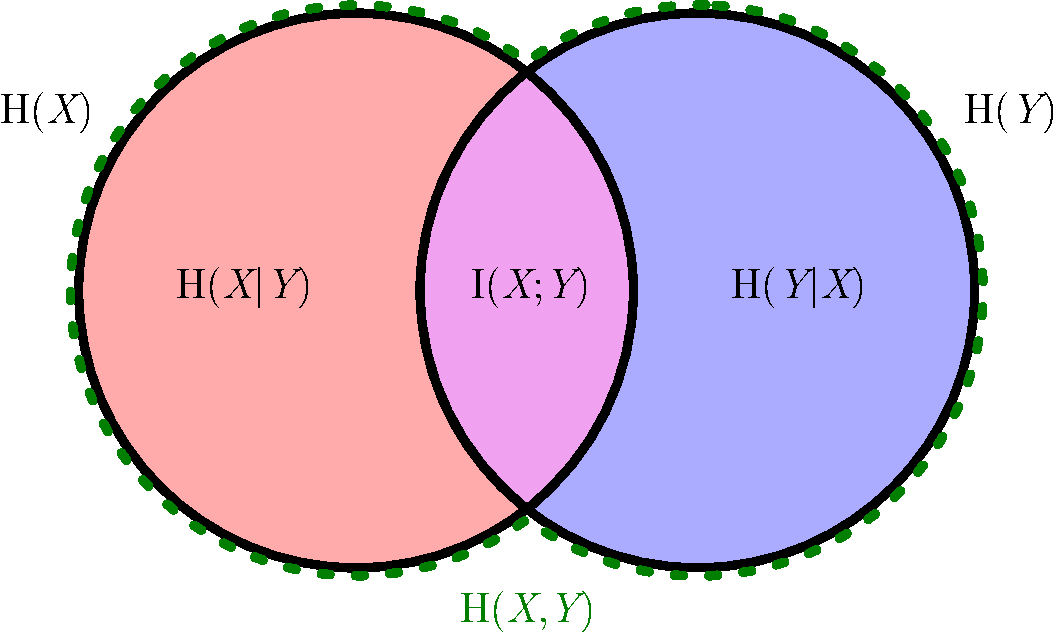
\includegraphics[scale=.5]{Entropy-mutual-information-relative-entropy-relation-diagram.pdf}
\caption{
\captionemph{Venn diagram of mutual information between $X$ and $Y$.}
The two black circles represent the entropies of $X$ and $Y$, $\HH(X)$ and $\HH(Y)$, and their total area (outlined in green) is the total joint uncertainty, $\HH(X, Y)$.
In the scenario depicted, $\HH(X)$ and $\HH(Y)$ are partially but incompletely redundant.
Consequently, the uncertainty of $X$ is reduced (but not expected to be zero) when $Y$ is known: the conditional entropy $\HH(X|Y)$ (red region) is smaller than $\HH(X)$, but is not empty.
The amount by which our expected uncertainty in $X$ is reduced, $\HH(X) - \HH(X|Y)$, is equivalent to the mutual information between $X$ and $Y$, denoted $\I(X;Y)$ and represented by the magenta region.
We can reason similarly about the other conditional entropy, $\HH(Y|X)$ (blue region).
% Reproduced (with modifications) from \href{https://commons.wikimedia.org/wiki/File:Entropy-mutual-information-relative-entropy-relation-diagram.svg}{Wikimedia Commons} (public domain).
}
\label{fig:bg_info_venn}
\end{figure}


\subsection{Applying information theory in practice}

Computing the mutual information between stimulus and response requires us to estimate $p(s)$, $p(r)$, and either $p(s|r)$ or $p(r|s)$ for every possible stimulus, $s$, and response, $r$.
The requirement to know $p(s)$ renders applying mutual information outside of a controlled environment all-but impossible.
If the subject is free moving, a prior over the set of potential stimuli it could be exposed to is very challenging to define.
However, within an experimental setting we can control the stimulus presentation such that there is only a finite set of unique stimuli, and the probability of each of them, $p(s)$, is defined by our experimental protocol.
In practice, $p(r|s)$ is much easier to derive than $p(s|r)$, and so we estimate $p(r)$ and $p(r|s)$.
As mentioned earlier, we must repeatedly present each stimulus so it is possible to estimate the response distribution $p(r|s)$ for each stimulus condition.

However, estimating these probabilities from the data can cause problems with our estimated mutual information.
Since we have only a finite number of samples, there will inevitably be inaccuracies in our probability estimates (the \textemph{limited sampling} problem).
Should we repeat the experiment, the natural variation in the samples we collect will result in statistical variance in our measured mutual information.
Moreover, the variation due to finite sampling may cause our response distributions to appear different for different stimuli, even when the underlying response generation process is the same for each stimulus.
Such problems produce an \textemph{over-estimation bias} in the computed mutual information compared with the ground truth.
For instance, if a particular response never occurs for a given stimulus presentation, a na{\"i}ve frequentist estimate of its probability would be $0$.
This would lead us to mistakenly conclude that it is impossible that a certain stimulus was presented if we observe this response, even if we could in fact have observed this combination of stimulus and response had we collected more samples.

Of even greater concern, the bias to the estimated mutual information can vary greatly depending on the choice of experiment or analysis framework.
One cannot draw comparisons between na{\"i}vely estimated mutual information values under different experimental criteria because the changes in the bias can completely dwarf the changes in the ground truth information value.
It is therefore necessary to estimate the bias on the na{\"i}ve mutual information value and make a correction to counteract it.


\subsection{Bias correction}
\label{sec:info-bias}

A number of techniques exist to correct for the bias in the mutual information estimation.
The simplest of these is to shuffle the data so that responses are paired with stimuli at random \citep{Optican1991}.
Unfortunately, this will often be a poor estimate of the bias \citep{Panzeri1996}, because there may be responses which never occur with certain stimuli.
Pairing stimuli and responses together at random inflates the set of unique responses to each stimulus above what is possible in practice, and as a consequence an estimate of the bias determined in this manner will be a pessimistic overestimate.

However, for a multi-dimensional response (where each stimulus presentation produces a response vector), shuffling provides an invaluable bias-correction technique.
Using the methodology of \citet{Montemurro2007}, we add an additional step to compute the noise entropy under the simplifying assumption that each dimension of $r$ is independent of the others.
Exploiting this, we have
\begin{equation}
p_\text{ind}([r_1,r_2,r_3,\cdots]|s) = p(r_1|s) \, p(r_2|s) \, p(r_3|s) \, \cdots
\end{equation}
and can compute $\HH_\text{ind}( R | S )$, the entropy under the independence assumption, directly from estimates of each $p(r_i|s)$ derived from the data.
This has very little bias compared with $\HH( R | S )$ since there are so many more samples --- the ratio of samples for unique response vectors to individual response elements rises exponentially with the dimension of the response vector.
One can alternatively estimate this entropy, $\HH_\text{ind}( R | S )$, from pseudo-response arrays by shuffling each element in the response vector conditioned on the stimulus, producing $\HH_\text{sh}( R | S )$.
Since this shuffling destroys information contained in the dependencies between elements in the response vector, this is an estimate of the same entropy value as $\HH_\text{ind}( R | S )$.
Except the bias on $\HH_\text{sh}( R | S )$ will be similar to the bias of $\HH( R | S )$ because each computation uses the same number of samples.
Consequently, we can estimate the mutual information between $S$ and $R$ using
\begin{align}
\I_{\text{sh}}(S;R)
   &= \HH( R ) - \left( \HH( R | S ) - \left( \HH_\text{sh}( R | S ) - \HH_\text{ind}( R | S ) \right) \right) \notag
\\ &= \HH( R ) - \HH( R | S ) + \HH_\text{sh}( R | S ) - \HH_\text{ind}( R | S )
,\end{align}
which has a much smaller bias than $\I_{\text{uncorrected}}(S;R)$.

An alternative method to correct for the bias is to decompose the measured mutual information as a power series in terms of $\nicefrac{1}{N}$, where $N$ is the number of trials recorded.
The $\nicefrac{1}{N}$ coefficient in the expansion depends only on the number of stimuli and number of possible responses \citep{Miller1955,Treves1995}.
This dominant term is a good estimate of the bias, and subtracting it from our uncorrected information value greatly improves its accuracy \citep{Treves1995}.
This works for a single-dimensional or multi-dimensional response, and is more accurate than shuffling for a single-dimensional response \citep{Panzeri1996}.
However, this term is dependent on the total number of potential responses for each stimulus.
Since some stimuli may not be able to elicit every response, this is smaller than the number of theoretically possible responses.
However as described above, some responses may be possible to produce but unobserved in the limited set of samples.
Consequently, the \ac{PT} bias-correction method of \citet{Panzeri1996} uses Bayesian statistics to estimate the actual number of potential responses.
This method was observed to be accurate provided there are at least \num{4} times as many repetitions of each stimulus as there are possible responses \citep{Panzeri2007}.

A second method of correcting the bias which uses a power series expansion is the \ac{QE} method of \citet{Strong1998}.
Here, the bias on the mutual information is assumed to be well approximated by a second order $\nicefrac{1}{N}$ expression,
\begin{equation}
\I_{\text{uncorrected}}(S;R) =
\I_{\text{true}}(S;R) + \frac{a}{N} + \frac{b}{N^2}
,\end{equation}
and the two free parameters, $a$ and $b$, are found by computing the information content with fractions of the full available dataset (\ie{} using $\nicefrac{N}{2}$ and $\nicefrac{N}{4}$ trials).
Since the two are built on the same assumptions \ac{QE} gives similar performance to \ac{PT}, but \ac{QE} requires more computational processing as it is fit empirically instead of derived analytically.

% Consider discussing Best Universal Bound (BUB) method (Paninski, 2003)

The \ac{NSB} entropy estimation method \citep{Nemenman2004} provides an alternative framework through which the bias can be minimised.
This method begins with a uniform prior and uses Bayesian inference to update the probability distribution given each sample in turn.
The result has less residual bias than the \ac{PT} or \ac{QE} methods, but at higher computational cost \citep{Panzeri2007}.

Each of these bias correction methods make a trade off between variability and bias.
Introducing more terms in order to reduce the bias invariably increases variability, but this is a price worth paying since the uncorrected bias is so prominent in the results.
Unless indicated otherwise, we will be using the \ac{PT} bias correction method when computing mutual information with a single dimensional response, and $\I_{\text{sh}}$ with \ac{PT} when using a multi-dimensional response vector.
In addition to this, we will repeat the mutual information calculation with shuffled stimulus-response pairing multiple times (typically 20 different shuffled pairings) with bias correction and use the average of the bootstraps to estimate the residual bias uncorrected by \ac{PT}.
The estimated residual bias is also removed from our reported mutual information between stimulus and response.


%------------------------------------------------------------------------------
\section{Neural correlations}
\label{sec:bg-corr}

When an individual is repeatedly presented with the same stimulus, a representation of the stimulus is formed within the brain of the individual.
One might expect that, should we eliminate variations in the environment such that an external stimulus is precisely the same --- an identical audio track is played without any background stimulus or a visual image is presented with the eyes held in place, for instance --- the activity within the associated sensory cortex would be identical on each repetition of the stimulus presentation.
However this is not the case.
Firstly, some stimuli, such as optical illusions and multistable perceptual phenomena induce unstable high-level representations in the brain \citep{Lumer1998,Sterzer2009,Watanabe2014}.
But this aside, for more classical typical stimuli (with only a single perceptual interpretation) the high-level representations of stimuli are stable, but the activity of each individual neuron is not.
On each successive presentation of a stimulus, the number of spikes elicited in response to the stimulus and the time at which each occurs may vary.
Precisely how a stable internal representation of a stimulus is constructed from the collection of unstable responses from individual neurons remains an open question actively researched within the theoretical neuroscience community.

Since neurons function in harmony and not in isolation, and the neural code is distributed across the population of many neurons, it is often important to consider how the behaviour of multiple neurons relate to one-another.
A simple way to do this is to measure the correlation between the outputs of pairs of neurons.

Although this is a less nuanced technique than using Shannon information to study the relationship between the neurons, measuring the correlation provides us with a much easier to use metric.
In particular, the amount of data needed to measure the mutual information between stimulus and response increases exponentially in the dimensionality of the response, which means it is impossible to compute the amount of information conveyed by the response of more than a handful of neurons.
In comparison, a simplistic interpretation of the correlation between the neurons can be performed with fewer trials.
However, as we discuss below, one must take into account the relationship between the signal and the noise correlation to correctly understand the impact of the neural correlations on the information contained by a collection of neurons.


\subsection{Signal correlations}
\label{sec:bg-sigcorr}

All other things being held constant, the response to a stimulus from an individual neuron will come from a fixed distribution.
Studying the average firing rate evoked in a single neuron in response to a collection of stimuli allows us to investigate the response profile of the neuron.
When the collection of stimuli vary parametrically, the distribution of responses for a given neuron with respect to this parameter is known as its \termemph{tuning curve}.

We can evaluate how similar the response profiles are for two neurons by computing their signal correlation.
To do so, we first find the average response from each neuron for a set of stimuli, $S$.
% Neural responses to repeated stimuli have high-variance, indicating a large amount of noise in the system.
Next, we calculate the Pearson correlation coefficient between the two sets of responses.
% By averaging the responses, we are sure to remove the effect of any correlations in the noise on the
In doing so, we treat each unique stimulus in $S$ as an independent sample of the relationship between the two neurons.
Some neurons behave similarly to each other in response to stimulation across a range of potential stimuli, and these pairs of neurons have correlated responses with respect to the input stimuli.

From an information theoretic perspective, neurons with high signal correlation will have high redundancy.
Of course, a redundant neural code is potentially useful as a method of error correction \citep[Chapter~1]{mackay2003information}, providing robustness against neuron death.
Having multiple neurons encoding the same information can improve accuracy by considering the population activity (the total or average of each neuron) instead of the individuals, and this may also permit a faster response time within the brain.
However, the prospective gain in performance when considering the responses from a set of neurons (redundant or not) depends on their noise correlations, and the relationship between the signal and noise correlation for the pair.
% Repetition is an inefficient method of error correction though \citep[Chapter~1]{mackay2003information}, and neuroscientists do not typically interpret groups of neurons to be duplicated instantiations of the same function of the stimulus.


\subsection{Noise response correlations}
\label{sec:bg-noisecorr}

Previously we noted that the response from a single neuron to a fixed stimulus is not fixed but effectively sampled from some stochastic distribution.
This internally-generated fluctuation in the neuronal response is referred to as noise.
When we consider a pair of neurons, the responses from each may vary independently over their two distributions; alternatively their responses may co-vary.
If the simultaneously measured responses from the pair of neurons are both higher than average on the same trials, and lower than average on the same trials, their noise is positively correlated.
Should the response from one neuron be consistently higher than average when the other is lower than average, we say their noise is negatively correlated.

To a certain extent, positive noise correlations between neighbouring neurons are inevitable, because they have correlated inputs.
Firstly, the path length (in the graphical sense of the number of separating nodes) between any given pair is likely to be short because neurons are preferentially connected to other neurons within their local vicinity.
Secondly, since there are more neurons in \ac{V1} than in the \ac{LGN} \citep{Kanitscheider2015}, the upscaling of the afferent sensory input makes noise correlations within \ac{V1} inevitable.

Intuitively, one can see that such noise correlations between pairs of neurons can inhibit the accuracy with which the stimulus is encoded in their activities.
Suppose that two neurons both respond monotonically more to stimuli of higher contrast.
Knowing their tuning curves and their current activity, we can decode the contrast of the current stimulus with some level of accuracy.
If the two neurons are independent of one another, knowing the activity of both will give us a more accurate and more precise estimate of the actual contrast of the stimulus.
But if the activity between the pair of neurons is positively correlated, the information conveyed from the pair of neurons is reduced --- when one gives an overestimate of the contrast from a by-chance elevated activity level, so does the other.
In contrast, negative correlations would enhance our decoding accuracy, for an overestimate from one neuron would more frequently be mitigated by an underestimate from the other.

However, this line of thinking only holds for a homogeneous population of neurons, where every neuron has its response drawn from the same distribution.
As illustrated in \autoref{fig:Averbeck2006a}, if a pair of neurons have positive signal correlation, then a positive noise correlation points in the direction distinguishing between the two stimuli, reducing the amount of information encoded by the pair of neurons.
If the pair of neurons have negatively correlated responses with respect to the stimuli, a positive noise correlation increases the amount of information encoded instead (\autoref{fig:Averbeck2006b}).

\begin{figure}[htbp]
\subfloat{\label{fig:Averbeck2006a}}
\subfloat{\label{fig:Averbeck2006b}}
\subfloat{\label{fig:Averbeck2006c}}
\centering
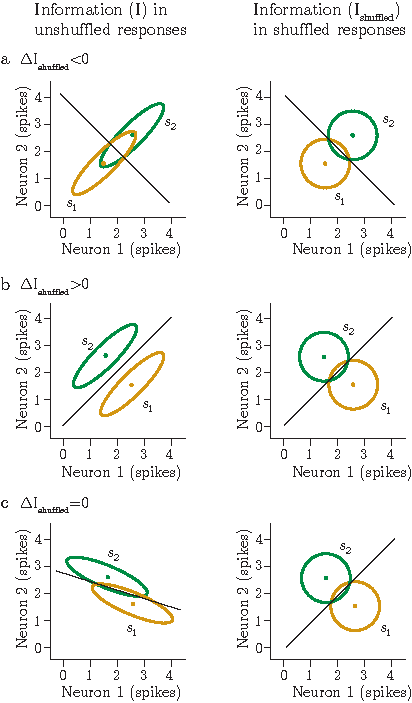
\includegraphics[scale=1.3]{Averbeck2006_Fig.pdf}
%
\caption{%
\captionemph{Effects of correlations on information encoding.}
We show the effect of positive noise correlations on the information encoded by two neurons that respond to two different stimuli in three scenarios.
The panels on the left show the original unshuffled responses, those on the right show the effect of shuffling the responses over trials to destroy the noise correlations.
Each ellipse indicates the \SI{95}{\percent} \acf{CI} for the responses.
Each diagonal line shows the optimal decision boundary --- responses falling above the line are classified as stimulus $2$ and responses below the line are classified as stimulus $1$.
\protect\subref{fig:Averbeck2006a}: A larger fraction of the ellipses lie on the ``wrong'' side of the decision boundary for the true, correlated responses than for the independent responses, so $I-I_\text{shuffled} = \Delta I_\text{shuffled} < 0$.
\protect\subref{fig:Averbeck2006b}: A smaller fraction of the ellipses lie on the wrong side of the decision boundary for the correlated responses, so $\Delta I_\text{shuffled}>0$.
\protect\subref{fig:Averbeck2006c}: The same fraction of the ellipses lies on the wrong side of the decision boundary for both the correlated and independent responses, so $\Delta I_\text{shuffled} = 0$.
% Reprinted/Adapted by permission from Macmillan Publishers Ltd: [JOURNAL NAME] (reference citation), copyright (year of publication)
Adapted by permission from Macmillan Publishers Ltd: \textit{Nature Reviews Neuroscience} \citep{Averbeck2006}, copyright 2006.
}
\label{fig:Averbeck2006}
\end{figure}


A similar line of reasoning can be considered for two neurons with offset tuning curves \citep{Franke2016}.
As shown in \autoref{fig:Franke2016}, when the two tuning curves are considered together we traverse a manifold in $2d$ space.
Noise correlations are a hindrance (information-limiting correlations, \citealp{Moreno-Bote2014}) only when the direction of noise correlation points in the same direction as the derivative of the tuning manifold, since this change is easily confused with a change in the parameter describing the manifold.
Whereas noise correlations which are orthogonal to the manifold are beneficial to the neural code, since the result has lower variability when projected onto the manifold than that of independently generated noise.
However, when the manifold forms a closed loop (as is the case with orientation tuning, shown in \autoref{fig:Franke2016}) the derivative of the tuning manifold processes through a full \SI{360}{\degree}, and the ideal noise correlation varies depending upon which stimulus signal is under consideration.

\begin{figure}[htbp]
\centering
\hspace*{\fill}
\subfloat[][Tuning curves for two model neurons.\label{fig:Franke2016a}]{%
    \includegraphics[scale=1.5]{%
10.1016-j.neuron.2015.12.037Figure6a1.eps}}
\hspace*{\fill}\hspace{.2cm}\hspace*{\fill}
\subfloat[][Pairwise responses traverse a manifold within $2d$ space.\label{fig:Franke2016b}]{%
    \includegraphics[scale=1.5]{%
10.1016-j.neuron.2015.12.037Figure6a2.eps}}
\hspace*{\fill}
\\
\subfloat[][The effect of noise correlations on decoding from the tuning manifold.\label{fig:Franke2016c}]{%
    \includegraphics[scale=1.5]{%
10.1016-j.neuron.2015.12.037Figure6b.eps}}
%
\caption{%
\captionemph{Impact of different structures of noise correlation upon population coding.}
\protect\subref{fig:Franke2016a}: Two model direction-selective neurons respond to different stimuli (dashed lines) according to tuning curves (solid grey curves), $f_1(\theta)$ and $f_2(\theta)$, with two direction preferences that differ by \SI{90}{\degree}.
\protect\subref{fig:Franke2016b}: The two tuning curves are represented as a solid grey line parametrized by the stimulus direction, $\theta$.
In the space of the two-neuron output, this grey line forms an informative subspace: the location of the pair response along the grey line yields information about the stimulus presented.
More precisely, for each stimulus, $\theta$, the tangent vector, $(f'_1(\theta),f'_2(\theta))$, defines the informative direction (arrows in colours corresponding to the stimulus values in the left panel).
\protect\subref{fig:Franke2016c}: For each stimulus presented, noise correlation distorts the cloud of two-neuron responses about the mean over trials; depending upon the geometry of this distortion with respect to the informative direction, it can either benefit or harm the coding accuracy.
Positive correlation in the pair ($c>0$) favours the reliability of coding with respect to the independent case ($c=0$), while negative correlation ($c<0$) is detrimental.
Specifically, when $c>0$, the responses for nearby stimulus directions overlap less, and, hence, coding is more reliable.
(Conversely, if the two tuning curves have similar preference, $c<0$ is favourable whereas $c>0$ is detrimental.)
More precisely, coding is favoured if the eigenvector of the covariance matrix parallel to the tangent vector, $(f'_1(\theta),f'_2(\theta))$, comes with a small eigenvalue; correlation then relegates the noise in the orthogonal, uninformative direction.
Ellipses are contours of equal probability, drawn at \num{2.5} standard deviations.
% Suitable acknowledgement to the source must be made, either as a footnote or in a reference list at the end of your publication, as follows:
% Reprinted from Publication title, Vol /edition number, Author(s), Title of article / title of chapter, Pages No., Copyright (Year), with permission from Elsevier
Reprinted from \textit{Neuron}, \citet{Franke2016}, Copyright (2016), with permission from Elsevier.
}
\label{fig:Franke2016}
%
\end{figure}
